\documentclass[letterpaper,11pt,notitlepage,fleqn]{article}

%\usepackage{nopageno} %gets rid of page numbers
\usepackage{alltt}                                           
\usepackage{float}
\usepackage{color}
\usepackage{indentfirst}
\usepackage{url}
\usepackage{balance}
\usepackage[TABBOTCAP, tight]{subfigure}
\usepackage{enumitem}
\usepackage{pstricks, pst-node}
\usepackage{geometry}
\geometry{textheight=9in, textwidth=6.5in} %sets 1" margins 
\newcommand{\cred}[1]{{\color{red}#1}} %command to change font to red
\newcommand{\cblue}[1]{{\color{blue}#1}} % ...blue
\usepackage{hyperref}
\usepackage{textcomp}
\usepackage{listings}
\usepackage{graphicx}
\usepackage{amsfonts}
\usepackage{amsmath}

% Code snippets color
\definecolor{dkgreen}{rgb}{0,0.6,0}
\definecolor{gray}{rgb}{0.5,0.5,0.5}
\definecolor{mauve}{rgb}{0.58,0,0.82}
\lstset{frame=tb,
  language=C,
  aboveskip=3mm,
  belowskip=3mm,
  showstringspaces=false,
  columns=flexible,
  basicstyle={\small\ttfamily},
  numbers=none,
  numberstyle=\tiny\color{gray},
  keywordstyle=\color{blue},
  commentstyle=\color{dkgreen},
  stringstyle=\color{mauve},
  breaklines=true,
  breakatwhitespace=true,
  tabsize=3
}
\lstdefinelanguage{diff}{
    morecomment=[f][\color{blue}]{@@},     % group identifier
  morecomment=[f][\color{red}]-,         % deleted lines 
  morecomment=[f][\color{green}]+,       % added lines
  morecomment=[f][\color{magenta}]{---}, % Diff header lines (must appear after +,-)
  morecomment=[f][\color{magenta}]{+++},
}
% End color
\def\name{Sam Quinn}

\parindent = 0.4444 in
\parskip = 0.2 in

\begin{document}
\begin{titlepage}
    \vspace*{\fill}

    \newcommand{\HRule}{\rule{\linewidth}{0.5mm}} % Defines a new command for the horizontal lines, change thickness here

    \center % Center everything on the page

    %----------------------------------------------------------------------------------------
    %TITLE SECTION
    %----------------------------------------------------------------------------------------

    %\includegraphics[scale=.5]{image.eps}
    \HRule \\[0.4cm]
    { \huge \bfseries Homework \#1}\\[0.4cm] % Title of your document

    %----------------------------------------------------------------------------------------
    %HEADING SECTIONS
    %----------------------------------------------------------------------------------------

    \textsc{\LARGE Oregon State University}\\[0.5cm] % Name of your university/college
    \textsc{\Large ECE 478 Network Security}\\[0.5cm] % Major heading such as course name
    \textsc{\large Spring 2016}\\[0.5cm] % Minor heading such as course title


    \HRule \\[1.5cm]
    %----------------------------------------------------------------------------------------
    %AUTHOR SECTION
    %------------------------------------ ----------------------------------------------------

    \begin{minipage}{0.4\textwidth}
        \begin{flushleft} \large
            \emph{Student:}\\
            \noindent \textbf{Sam \textsc{Quinn}} \\ % Your name
            {\small Quinnsa@Oregonstate.edu}
        \end{flushleft}
    \end{minipage}
        ~
        \begin{minipage}{0.4\textwidth}
            \begin{flushright} \large
                \emph{Professor:} \\
                \noindent \textbf{Dr. Attila A \textsc{Yavuz}} \\ % Supervisor's Name
                {\small Attila.Yavuz@oregonstate.edu}
            \end{flushright}
        \end{minipage}\\[3cm]

        %----------------------------------------------------------------------------------------
        %DATE SECTION
        %-----------------    -----------------------------------------------------------------------

    {\large \today}\\[3cm] % Date, change the \today to a set date if you want to be precise

    %----------------------------------------------------------------------------------------
    %LOGO SECTION
    %------   ----------------------------------------------------------------------------------

    
\includegraphics[scale=0.5]{coe.eps}\\[1cm] % Include a department/university logo - this will require the graphicx package

    %----------------------------------------------------------------------------------------

    \vfill % Fill the rest of the page with whitespace



\end{titlepage}

\tableofcontents
\newpage
\section{[24] Merkle Hash Tree}
%\Tree[.1$\Box\Box\Box\Box$ [.2$\Box\Box\Box\Box$ [.4$\Box\Box\Box\Box$ $\Box\Box{b1}\Box$\\8 $\Box\Box\Box{b2}$\\9 ][.5$\Box\Box\Box\Box$ $\Box\Box\Box{b3}$\\10 $\Box{b4}\Box\Box$\\11 ]][.3$\Box\Box\Box\Box$ [.6$\Box\Box\Box\Box$ ${b5}\Box\Box\Box$\\12 $\Box\Box{b6}\Box$\\13 ][.7$\Box\Box\Box\Box$ $\Box{b7}\Box\Box$\\14 ${b8}\Box\Box\Box$\\15 ]]]
\begin{center}
    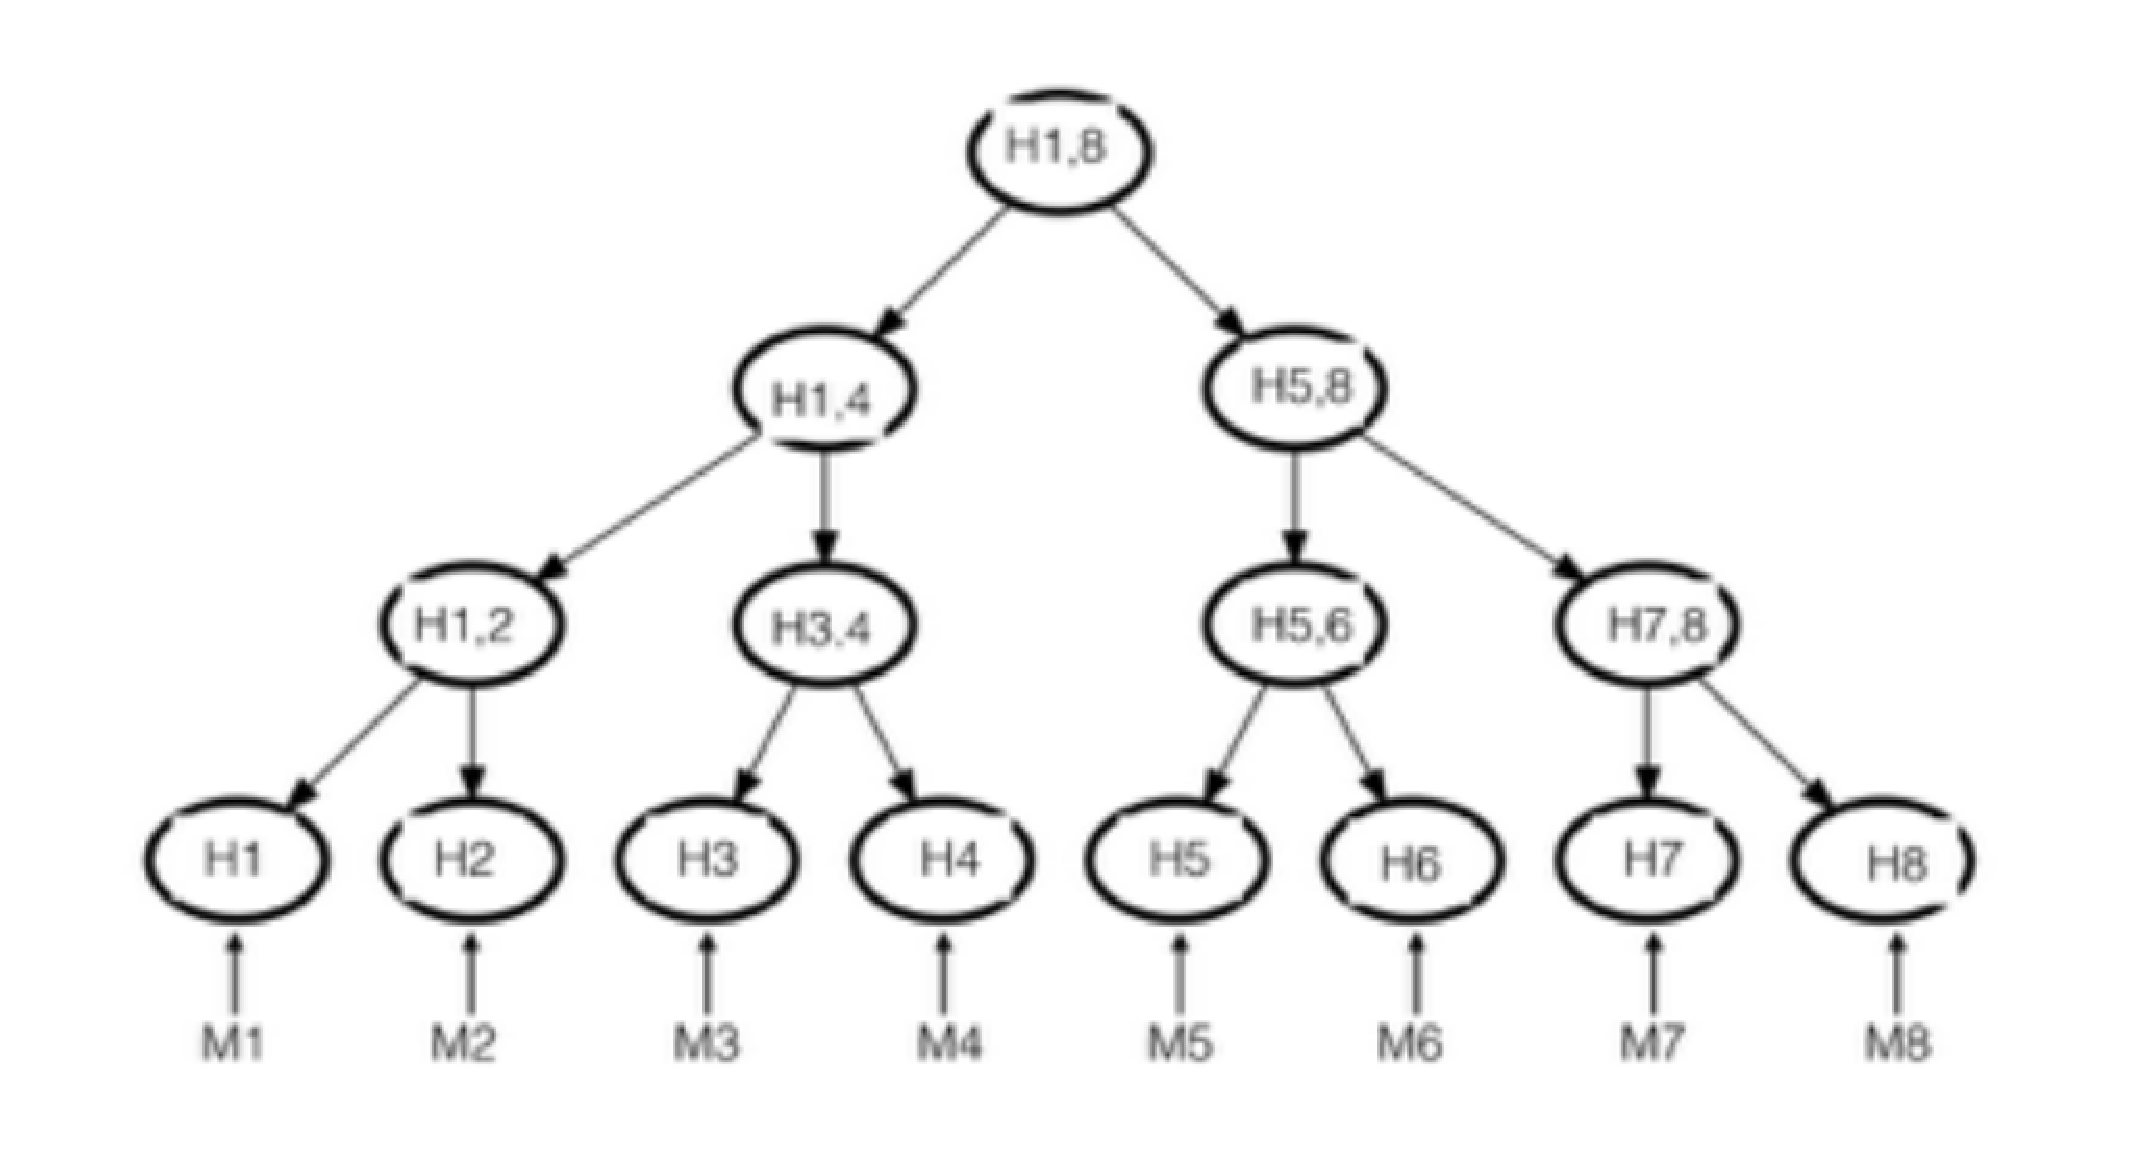
\includegraphics[scale=0.5]{tree.eps}
\end{center}

\noindent \textbf{Suppose a sender S uses this Merkle hash tree to authenticate these messages to a receiver R. What should be done before this tree can be used?}

Before the Merkle hash tree is able to be sent the root of the tree (H1,8) must be authenticated. This is typically done through a digital signature of pre-distribution. If the root is not authentication by a trusted source before the hash tree is used then all the proceeding data could also become compromised if a fraudulent tree matches the top node. 

\noindent \textbf{[8] How would one authenticate message 4?}

To authenticate a message trough a Merkle tree you must complete the entire path to the root. In the tree displayed above you would need to compute H3 and H4 to get H3,4 and then you would need H1,2 and H3,4 to get H1,4. Then the last step would be to get H5,8 which combined with H1,4 will give you H1,8 and thus be able to verify the tree and if message M4 was tampered with or not.


\noindent \textbf{[8] Merkle hash trees have an additional level of hash in the leaves. Is this necessary? Why?}

The additional level of hashes is not necessary but prevents unnecessary disclosure. To authenticate a message the verifier would either need to know the message to calculate the parent node or the verifier could use a hash of the message. If the verifier does not need to know the adjacent messages it is a benefit to have another level of hashes. 

\noindent \textbf{[8] What are the necessary conditions for a set of data to be authenticated by Merkle-tree? Please provide at least two example application where Merkle-tree with proper data type can be used.}

The sender must have the space to store the whole tree, the receiver needs space only to store the hashes of each node. The root node also needs to be trusted by both the sender and receiver. 

Merkle trees are present in cryptocurrencies. Each block of Bitcoin's public ledger is designed as a Merkle tree where each transactions hash is added the tree and can be verified very quickly. This provides authentication on each individual transaction.

Peer to peer networks use Merkle trees to guarantee that the data has not been corrupted during transmission. P2P networks with the Merkle trees can also verify that the other peers are not tampering with the data by checking the received block to the tree. 


\section{[24] Cryptographic hash functions and their use in one-time/multiple time signatures}

\noindent \textbf{[12] Let L be the number of messages, t is the number of bits to be signed in a message, and |f| is the bit-length of one-way function. Describe Lamport One time signature variant I, II, III, IV, VI, and VII (excluding V) . For each variant, describe the its algorithm, its performance in terms of security and efficiency,  and what are the key sizes and what is its storage complexity. For example, for one variant, you might want to mention what is the computational complexity for the
efficiency  of the algorithm and what is the security trade-off you must pay in order to achieve that efficiency. You must also mention what is the storage complexity of the public and private key in Big O.} 

\begin{description}
    \item [Variant I] \hfill \\ 
        Algorithm:\hfill \\ 
        \textit{Variant I} will create a random public and private key for both 1's and 0's for each bit in the message. Every bit in the message will be signed. \hfill \\
        Performance:\hfill \\ 
        \textit{Variant I} is considered secure based on the fact that the signature leverages the OTP property. The size of the keys are where this variant is lacking. Since the keys are $|sk|=|pk|=2|h|\ast|h|$ and $\sigma = |h|\ast|h|$ 
%\indent\indent $m = (m_{i},\dots,m_{n}) \sigma = (x_{1}m_{1},\dots,x_{n}m_{n})$ \\
%\indent Verify:\\
%\indent\indent if $f(x_{1}, m_{i})=y_{i}m_{i}$  $\forall$ $i$ return $1$ else $0$ \\
    \item [Variant II] \hfill \\
        Algorithm:\\
        \textit{Variant II} is similar to \textit{Variant I} however only the 1's are signed in this scheme.\\
        Performance: \\
        \textit{Variant II} by signing only 1's or 0's is able to reduce the key size by approximately half from \textit{variant I}. If any bits are flip the checksum will flag them. $|sk|=|pk|=|h|\ast|h|$ and $\sigma = |h|\ast|h|$
    \item [Variant III] \hfill \\
        Algorithm:\\
        \textit{Variant III} takes advantage of a cryptographic pseudo random number generator to allow the private key to be a constant size. \\
        Performance:\\
        Because \textit{variant III} through the use of hash-chains allows the private key remain constant, however there is more computation involved making the trade-off between storage and computation. \\
    \item[Variant IV] \hfill \\
        Algorithm:\\
        \textit{Variant IV} takes the idea of hash chains from \textit{variant III} and creates a 2D hash chain.  \\
        Performance:\\
Just as before using hash chains take less storage while the computation is increased but now the size and computation is increased but the data is less vulnerable to attacks. \\

\item[Variant VI] \hfill \\
    Algorithm:\\
        \textit{Variant VI} sends the public key with the signed message for every message.\\
        Performance:\\
        This is a constant function based on the size of the message and public key. The only performance drop is that if a packet is dropped, since \textit{variant VI} is stateful it requires the next public key with each packet. \\

    \item [Variant VII] \hfill \\
        Algorithm:\\
        \textit{Variant VII} takes the constant time algorithm from \textit{variant VI} but addresses the problem of dropping packets. Robustness through out packet drop is achieved by including multiple public keys in the signature. \\
        Performance:\\
This variant takes more communication overhead to achieve greater network reliability. If a packet is lost the real-time authentication could hiccup and should be accounted for in choosing the correct variant. \\

\end{description}

\noindent \textbf{[12] One-time/multiple signatures, after many years, started gain a new traction in  the  research  community.  What  is  the  main  reason  behind  this?  Compared traditional cryptographic methods  (e.g., RSA, ECDSA), what  is  the main security advantage of multiple-time signatures and why they are more secure?}  

One thing that One-time and Multiple signatures are really good at is protecting against quantum computers and their advantages in breaking traditional cryptographic methods. The reason that many cryptographic methods are not quantum restraint is that they use very complex math to gain security with either discrete logarithm problem or an elliptical curve. Quantum computers are able to calculate many more possibilities in a relatively small amount of time reducing the over all
security of the schemes that use these math problems. One-time and multiple signatures have the property of one time pad where the keys are uniformly random and do not rely on any mathematical problems that quantum computers could take advantage of. 

\section{[48] RSA encryption and digital signatures}

\noindent \textbf{[8]  What  is  the  role  of  Euler-Function,  Extended  Euclid  Algorithm  and  Fermat Little  Theorem  in  RSA  encryption?  Explain  the  role  of  each  by  showing  the specific step in RSA encryption and decryption process.}

The \textit{Euler totient function} or $\phi(n)$ is the set of numbers that are relatively prime to $n$. The Euler totient is crucial in RSA with the creation of the variables $e$ and $d$.\\
\begin{center}
    \begin{tabular}{l}
        $\phi(n) = |\mathbb{Z}_{n}^{*}|$ \\
        $n\ \leftarrow$ if $p,q$ are prime $(p \neq q)$ then $\phi(pq) = (p-1)(q-1)$
    \end{tabular}
\end{center}

The \textit{Extended Euclidean algorithm} is a way for finding the GCD. RSA needs to satisfy certain properties that require having a GCD of 1, for example $GCD(e,\phi(n)) = 1$\\
\begin{center}
    \begin{tabular}{l}
        $gcd(p,q) = 1$ Then for all $u,v$ there is a solution for $x$ in \\
        $x = u$ $mod(p)$ \\ 
        $x = v$ $mod(p)$ 
    \end{tabular}
\end{center}

The \textit{Fermat Little Theorem} is $a^{p-1} \equiv 1$ $mod(p)$ but in its application to RSA it is used to produce the $d$ value, which is the inverse of $e$.\\
\begin{center}
    \begin{tabular}{l}
        $d \ast e \equiv 1\ (mod\ \phi(pq))$
    \end{tabular}
\end{center}

\noindent \textbf{[8] Using Euclid’s algorithm (Not extended, but just Euclid), calculate the $g$ $gcd(16261,  85652)$.  Using  Fermat’s  little  theorem,  compute  $3^{31}  (mod\ 7)$  (Hint: Decompose the exponent)} 

To find the GCD using Euclid's algorithm you must:
\begin{center}
    \begin{tabular}{l}
        $gcd(16261, 85652)$\\
        $85652 = 16261 \ast 5 + 4347$\\
        $16261 = 4347\ast 3 + 3220$ \\
        $4347 = 3220\ast 1 + 1127$ \\
        $3220 = 1127\ast 2 + 966$ \\
        $1127 = 966\ast 1 + 161$ \\
        $966 = 161\ast 6 + 0$ \\
        \textbf{GCD:} $161$\\
    \end{tabular}
\end{center}

To find $3^{31} \equiv ?$ $(mod\ 7)$ the following takes place:
\begin{center}
    \begin{tabular}{l}
        $3^{6} \equiv 1$ $(mod\ 7)$\\ \\
        $3^{31} \equiv 3^{(5 \ast 6)}\ast 3^{1}$ $(mod\ 7)$\\
        $3^{31} \equiv 1^{5}\ast 3^{1}$ $(mod\ 7)$\\
        $3^{31} \equiv 1 \ast 3$ $(mod\ 7)$\\
    \end{tabular}
\end{center}

\noindent \textbf{[8]  In  RSA,  public  key  e  can  be  smaller  than  the  private  key  d.  What  are  the performance  and  security  implications  of  this?  What  should  be  considered  for selecting public exponent e as a security metric?}

The reason that the public key $e$ can be smaller than the private is that everything is within the cyclic group of $Z_{n}^{*}$ so any number raised to the $e$ will be with in the bounds of $1-\phi(n)$.
Having a smaller $e$ allows for the data to be encrypted faster since the exponential is the slowest aspect of the RSA algorithm, the smaller the number the quicker the data can be encrypted. 

It has been proven that you should not use too small of an $e$ as they have been broken, for example $e=3$ and $e=7$. This attack is considered a small exponent attack. An adequate size of key for $e$ would be $e=2^{16}+7$. One note to take during the creation of $e$ is that it should not have any common factors with $\phi(n)$.   

\noindent \textbf{[8]  In  RSA  encryption  and  signatures,  the  use  of  private/public  key  pair  between sender  and  verifier  is  swapped.  Why  this  is  the  case?  (Hint:  Think  about  the purpose  of  signatures  and  encryption.  Also,  think  about  the  purpose  of authentication and its difference from encryption)}

The reason that the keys are swapped is for authentication. In RSA the data is raised to the $e$ and $d$ exponents that are inverses of each other. The only difference between the two is that the private key $d$ should never be exposed to anyone other than the owner. When data is digitally signed it should provide authenticity of the owner so the private key $d$ is used so it can be verified by the public key $e$ by anyone.  

\noindent \textbf{[8]  In  RSA  signatures,  randomness  was  introduced  during  the  signing  process using  Coron’s  Full  Domain  Hash  Function.  What  is  the  objective  of  this randomness?} \textit{Please again use Google Scholar to look up JS Coron’s paper on full domain hash  function. You may want  to  look Bellare’s paper on  full domain hash function.  Please  note  that  full  domain  hash  function  IS  NOT  an  RSA-based signature scheme.}

The randomness is introduced to to obtain a better security bound and tighten security. From Bellare's paper, trapdoor permutations can be included to a scheme as a random oracle heuristic. Randomness within an encryption scheme also helps achieve IND-CPA security since the resulting ciphertext will be indistinguishable even if the same data is encrypted twice~\cite{Hohen}~\cite{Coron}. 


\noindent \textbf{[8]  Textbook  implementation  of  RSA    is  subjected  to  timing-based  side-channel attacks. Explain why  (Hint:  see how  square  and multiply  algorithm works  and  tie this  to  a  side-channel  attack).  Describe  a  simple  blinding  technique  that  can prevent this basic side-channel attack. This technique is also called masking.}

For an adversary to perform a side-channel attack requires the adversary to attack aspects apart from the actual encryption scheme. RSA requires certain mathematical functions to encrypt and decrypt data. Each of the mathematical operations take a slightly different time, an adversary may use this time discrepancy to their advantage by calculation ranges of numbers and analyse the time took to get an estimate of what the internal secret variables are. 

\section{[24] ORAM}

\noindent \textbf{[6] What is the basic formal security definition of ORAM? Please go on Google Scholar and find the Path-ORAM paper by Emil Stefanov et al.} 

Oblivious RAM (ORAM) algorithms, allow client to conceal its access pattern to the remote storage by continuously shuffling and re-encrypting data as they are accessed. ORAM algorithms ensure that the adversary has negligible probability of learning anything about the true (logical) access patterns~\cite{Stef}.  


\noindent \textbf{[4] What is IND-CPA encryption? Give its formal definition based on symmetric encryption.}

IND-CPA encryption is an encryption scheme that satisfies IND-CPA security. IND-CPA security stands for Indistinguishable Chosen Plaintext Attack, meaning that if an adversary had the opportunity to choose ciphertext there would still be no way for them to determine which is theirs compared to completely random output. 

\noindent \textbf{[4] Why IND-CPA encryption is required in order for ORAM to work?}

IND-CPA is required because an adversary could have their chosen cipher text moved to a spot in memory and attempt to try to decrypt it. Also it is essential for the data to be indistinguishable from all the other data. 

\noindent \textbf{[10] Give a basic Path ORAM tree with 8 items, where b1,…,b8 represent blocks to be accessed (assume stash size = 4). Denote each intermediate node with a number (see ORAM slides for an example). On this Path ORAM tree, why is accessing the same block arbitrary number of times yield indistinguishable access patterns?} 
\includegraphics[scale=.22]{oram.eps}\\
\indent The reason access patterns cannot be analyzed is due to the fact the whole path that the goal node exists on is downloaded. If \textbf{b2} needs to be accessed then the path with \textbf{b1},\textbf{b3}, and \textbf{b8} would also be downloaded obscuring the actual block that is wanted. 
\noindent \textbf{How is this achieved?}
\begin{description}
    \item [Why IND-CPA encryption plays a role on this?] \hfill \\
        As stated above ORAM needs IND-CPA since it needs all data to be indistinguishable even if the adversary has the opportunity to choose their own ciphertext. 
    \item [Which  step  of  Path-ORAM  ORAM  algorithm  (in  addition  to  IND-CPA aspect) is vital to achieve indistinguishable access patterns?] \hfill \\
        The use of a stash is vital to to protecting the physical access patterns of the data. The stash is able to shuffle the location of the retrieved data when putting it back into memory. 
\end{description}

\medskip
\bibliography{quinnsaHW2}
\bibliographystyle{ieeetr}
\end{document}
